\begin{frame}
	\frametitle{O que é Segurança Pública}
	O ministério da justiça\cite{seguranca-publica} define como:
	\begin{itemize}
		\item \textbf{O que é:}
		Previnir e controlar manifestações da criminalidade
		e da violência, efetivas ou \textbf{potenciais}.
		\item \textbf{Responsabilidade de:}
		Órgãos estatais e à Comunidade.
	\end{itemize}
\end{frame}

\begin{frame}
	\frametitle{Soluções Empregadas Atualmente (Brasil)}
	\begin{itemize}[<+->]
		\item Lei seca;
		\item Cinto de segurança;
		\item Cadeirinha infantil;
		\item Capacete;
		\item Regulamentação e fiscalização de velocidade
		máxima;
		\item \textbf{Câmeras de monitoramento}.
 	\end{itemize}
\end{frame}

\begin{frame}
	\begin{figure}[h]
		\caption{COI São José dos Campos - 2017}
		\centering
		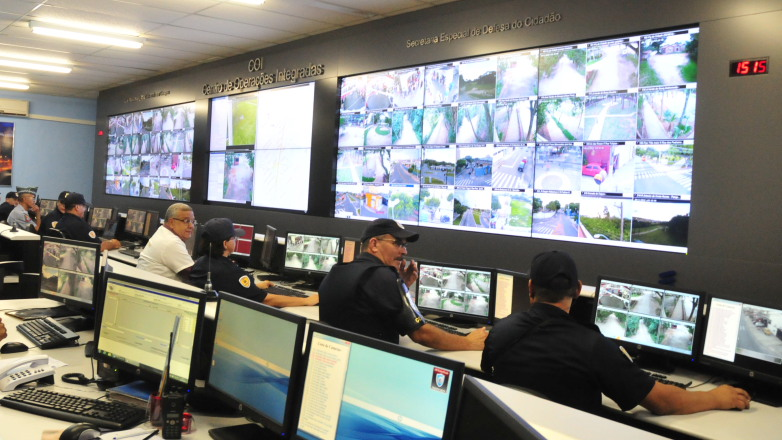
\includegraphics[width=1\textwidth]{imagens/coi}
	\end{figure}
\end{frame}

\begin{frame}
	\frametitle{O que é \textit{Machine Learning}?}
	\textit{[Machine  Learning  is  the]  field  of  study  that  gives  computers  the  ability  to  learn
	\textbf{without} being explicitly programmed.}
	—Arthur Samuel, 1959
\end{frame}

\begin{frame}
	\frametitle{Tipos de \textit{Machine Learning}}
	Uma \textbf{ML} pode ser categorizada\cite{machine-learning} em:
	\begin{itemize}[<+->]
		\item Por Supervisão:
			\begin{itemize}[<+->]
				\item Supervisionado;
				\item Não Supervisionado;
				\item Semi-supervisionado;
				\item Aprendizado por Reforço.
			\end{itemize}	
		\item Por Método de Aprendizado:
			\begin{itemize}[<+->]
				\item Incremental;
				\item Batch File.
			\end{itemize}
		\item Por Modelagem:
		\begin{itemize}[<+->]
			\item Comaparação;
			\item Detecção de Padrões.
		\end{itemize}
	\end{itemize}	
\end{frame}